
Una vegada havia implementat la distància de Férchet per poder avaluar el rendiment dels models, vaig arribar a una clara conclusió:

Els models que tenen implementada la funció no-lienal són més eficients. 

Arribo a aquesta conclusió, ja que els models sense la funció no arriben a estabilitzar-se, és a dir, no arriben al punt d'equilibri. En canvi, els models que si la presenten si ho fan. Arribar al punt d'equilibri ens garanteix que les imatges que generen seguin òptimes indefinidament. Per molt més que el model segueixi optimitzant-se, sempre donarà els mateixos resultats.


Els models que no presenten la funció, no assoleixen el punt d'equilibri, com que la fidelitat de les imatges oscil·la És a dir, poden arribar a generar imatges correctament, però no ho fan indefinidament, al cap d'unes interaccions la semblança de les imatges generades amb les reals no és significativa.

Aquest problema no és causat pel discriminador, això és veritat perquè la variable independent de l'experiment, és el circuit quàntic del generador. Per tant, és el factor que té més possibilitat de ser el causant d'aquest comportament. No sé molt bé la causa exacta, però està clar que el mesurament parcial té un impacte. Tot i que hi ha excepcions, a vegades els models sense la funció no experimenten aquesta oscil·lació. Però cal remarcar que les vegades que passa són notablement més altes que les que no passa. Com es pot veure amb les dades de la taula \ref{tab:oscilations}

\begin{table}[]
	\resizebox{\textwidth}{!}{%
		\begin{tabular}{c|c|c}
			\hline
			& Presenta oscil·lació & No Presenta oscil·lació \\
			\hline
			Amb Funció No-Lineal & 0 & 6 \\
			\hline
			Sense Funció No-Lineal& 5 & 1 \\
			\hline
		\end{tabular}
	}
	\caption{Les dades provenen d'un total de 6 models, 3 d'ells amb un total de $700$ epoch i els altres 5 amb un total de $550$. El nombre d'interaccions no hauria d'afectar de cada manera les dades. Degut si hi ha una oscil·lació, es pot veure clarament a partir de les $400$ iteracions. Amb les dades es pot veure que és més probable que un model sense la funció lienal presenti una oscil·lació. Cal notar que cap model amb la funció ha tingut una oscil·lació. Les gràfiques que corresponen a cada model es poden veure en la figura \_.}
	\label{tab:oscilations}
\end{table}

\begin{figure}[H]
	\begin{subfigure}[b]{.32\linewidth}
		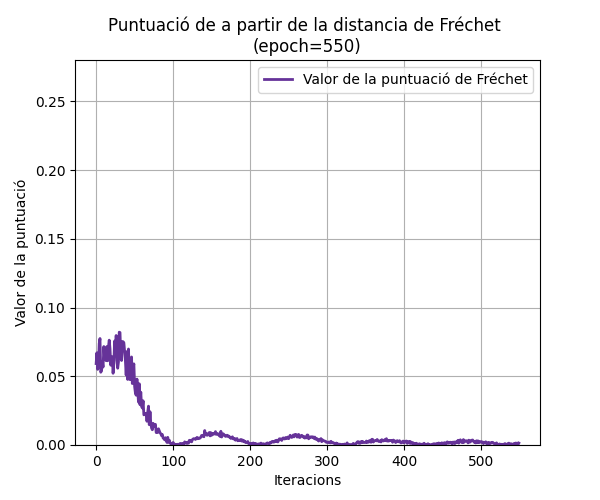
\includegraphics[width=\linewidth]{figures/data/FD_score_1.png}
		\caption{}
	\end{subfigure}
	\begin{subfigure}[b]{.32\linewidth}
		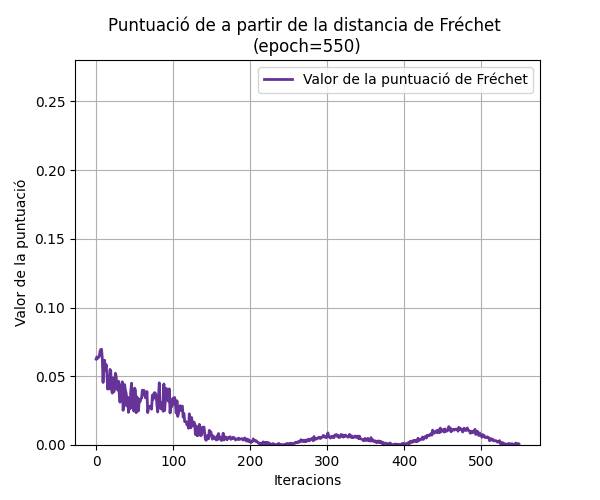
\includegraphics[width=\linewidth]{figures/data/FD_score_2.png}
		\caption{}
	\end{subfigure}
	\begin{subfigure}[b]{.32\linewidth}
		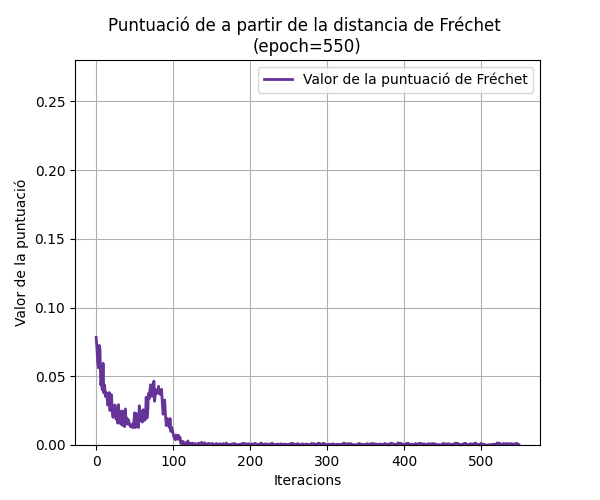
\includegraphics[width=\linewidth]{figures/data/FD_score_3.png}
		\caption{}
	\end{subfigure}
	
	\begin{subfigure}[b]{.32\linewidth}
		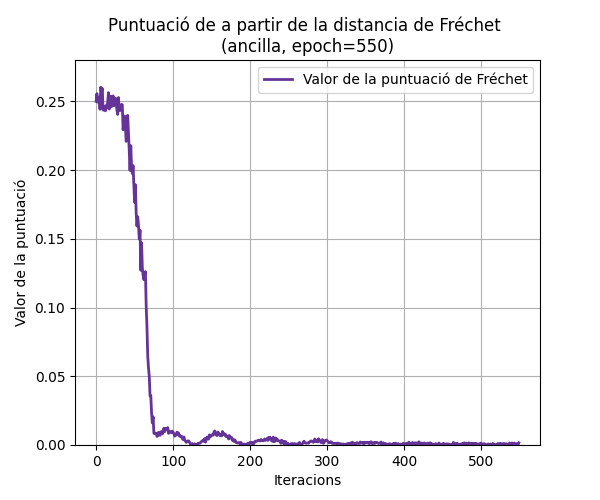
\includegraphics[width=\linewidth]{figures/data/FD_score_A1.png}
		\caption{}
	\end{subfigure}
	\begin{subfigure}[b]{.32\linewidth}
		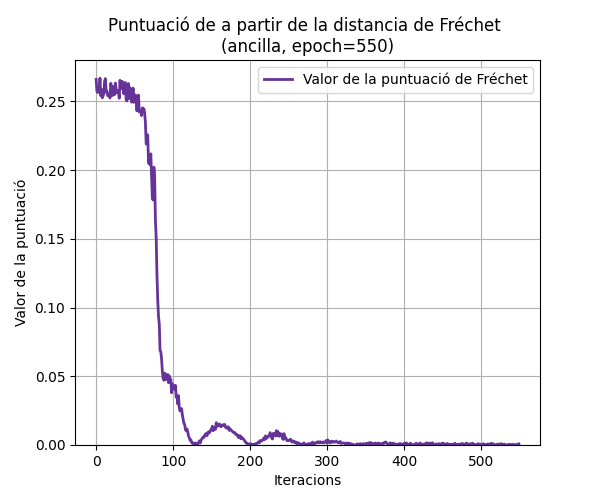
\includegraphics[width=\linewidth]{figures/data/FD_score_A2.png}
		\caption{}
	\end{subfigure}
	\begin{subfigure}[b]{.32\linewidth}
		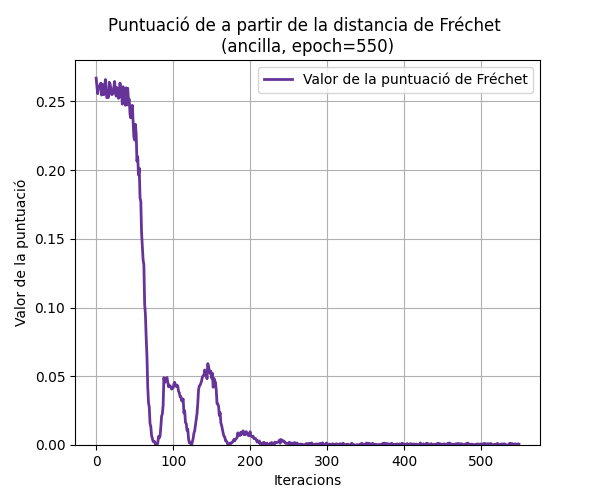
\includegraphics[width=\linewidth]{figures/data/FD_score_A3.png}
		\caption{}
	\end{subfigure}
	\caption{Totes les gràfiques corresponen a models que s'ha executat al llarg de $550$ iteracions. Les figures \textbf{A}, \textbf{B} i \textbf{C}, corresponen a models sense la funció lineal. L'únic d'ells que no presenta una oscil·lació és el \textbf{C}. Les gràfiques sense la funció es poden comparar a les d'abaix, les quals representen models amb la funció implementada. Els models han estat creats per parelles, les quals estan organitzades verticalment. És a dir, les gràfiques \textbf{A} i \textbf{D} representen models que tenen els mateixos paràmetres inicials. El mateix passa amb \textbf{B} i \textbf{E} i amb \textbf{C} i \textbf{F}.}
\label{fig:550_SD_score}
\end{figure}

\begin{figure}[H]
	\begin{subfigure}[b]{.32\linewidth}
		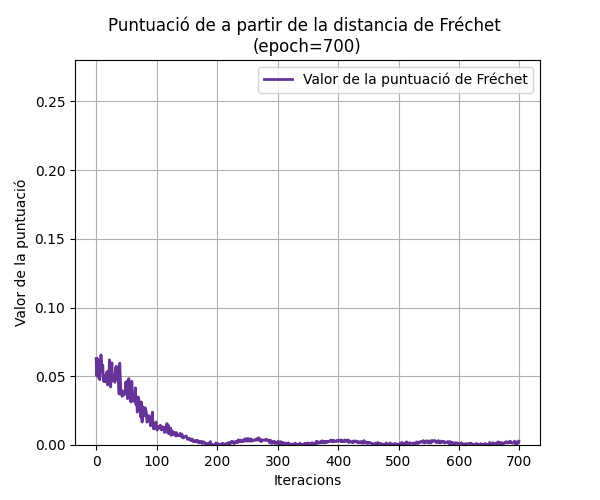
\includegraphics[width=\linewidth]{figures/data/FD_score_4.png}
		\caption{}
	\end{subfigure}
	\begin{subfigure}[b]{.32\linewidth}
		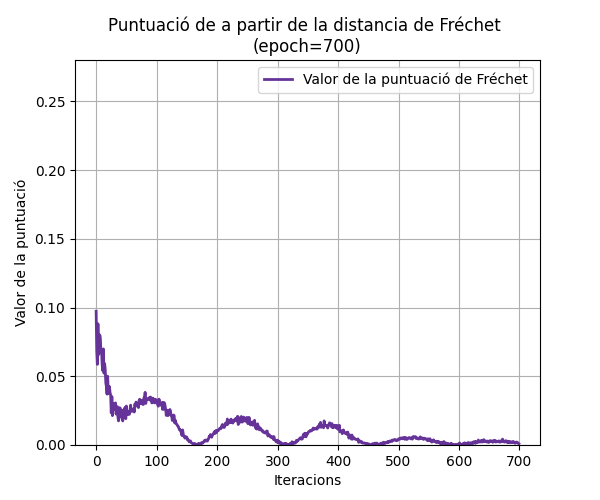
\includegraphics[width=\linewidth]{figures/data/FD_score_5.png}
		\caption{}
	\end{subfigure}
	\begin{subfigure}[b]{.32\linewidth}
		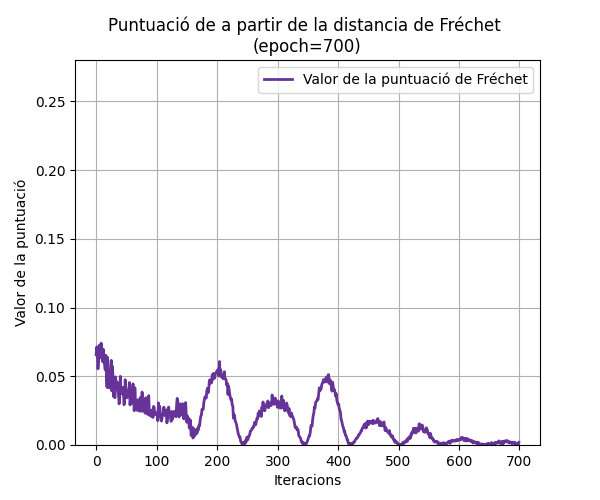
\includegraphics[width=\linewidth]{figures/data/FD_score_6.png}
		\caption{}
	\end{subfigure}
	
	\begin{subfigure}[b]{.32\linewidth}
		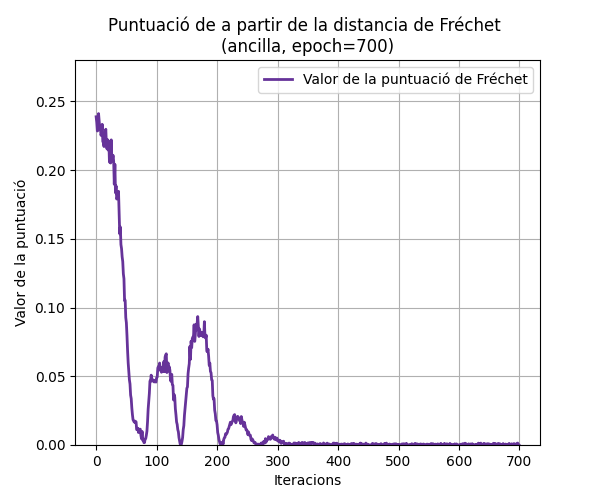
\includegraphics[width=\linewidth]{figures/data/FD_score_A4.png}
		\caption{}
	\end{subfigure}
	\begin{subfigure}[b]{.32\linewidth}
		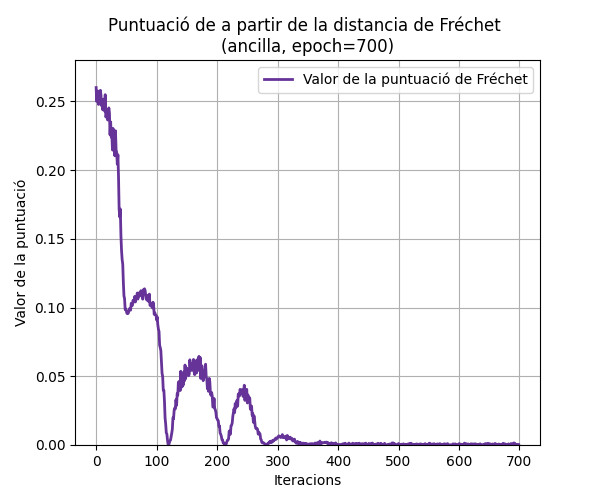
\includegraphics[width=\linewidth]{figures/data/FD_score_A5.png}
		\caption{}
	\end{subfigure}
	\begin{subfigure}[b]{.32\linewidth}
		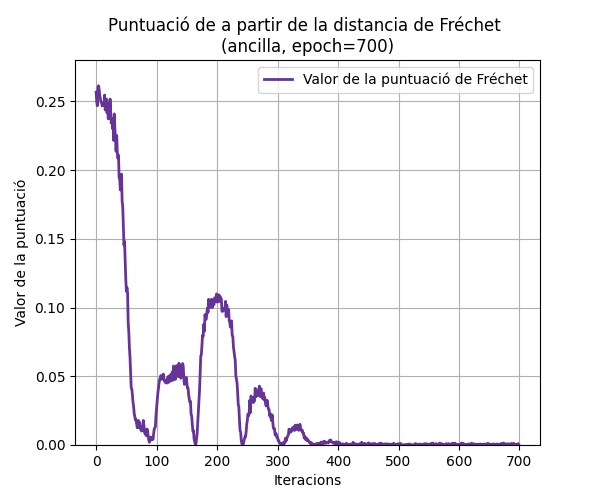
\includegraphics[width=\linewidth]{figures/data/FD_score_A6.png}
		\caption{}
	\end{subfigure}
	\caption{Aquestes gràfiques corresponen a models que s'han executat al llarg de $700$ iteracions. Estan organitzades igual que les gràfiques de la figura \ref{fig:550_SD_score}. En aquests casos, com es pot observar tots els models sense la funció no-lineal presenten les oscil·lacions. No obstant en la gràfica \textbf{A}, aquesta es molt feble. Per veure com afecten les oscil·lacions es pot veure la figura, on estan representades les últimes imatges que han generat els models que corresponen les gràfiques d'aquesta figura.}\todo{aquestes figures tenen el terme [H], veure si es útil}
	\label{fig:700_SD_score}
\end{figure}

\begin{figure}[H]
	\begin{subfigure}[b]{.32\linewidth}
		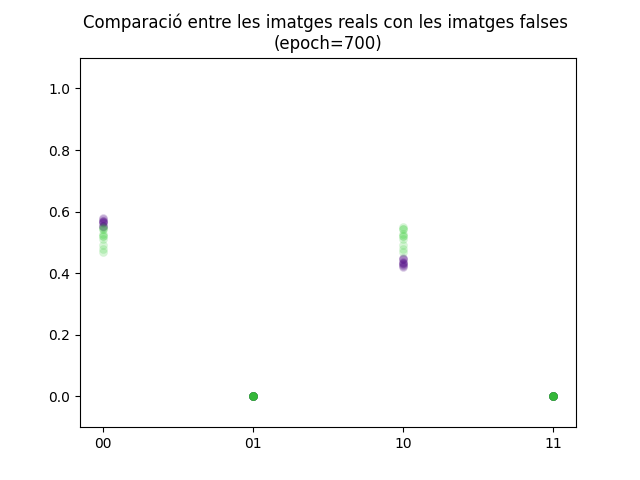
\includegraphics[width=\linewidth]{figures/data/scatter_plot_4.png}
		\caption{}
	\end{subfigure}
	\begin{subfigure}[b]{.32\linewidth}
		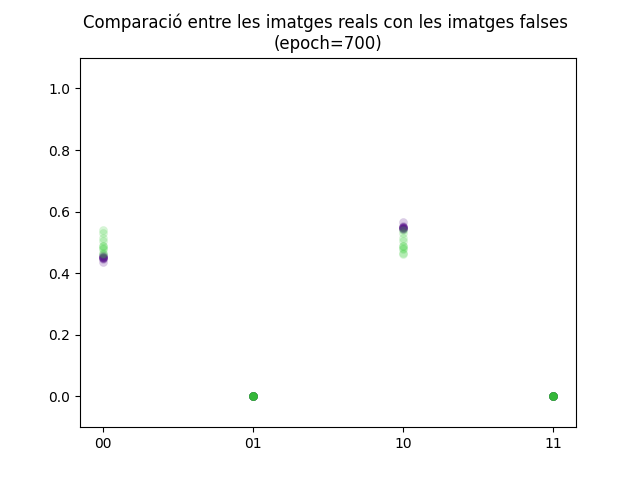
\includegraphics[width=\linewidth]{figures/data/scatter_plot_5.png}
		\caption{}
	\end{subfigure}
	\begin{subfigure}[b]{.32\linewidth}
		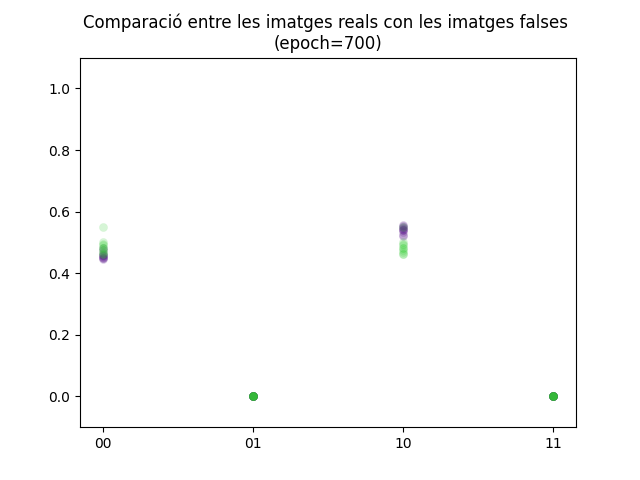
\includegraphics[width=\linewidth]{figures/data/scatter_plot_6.png}
		\caption{}
	\end{subfigure}
	
	\begin{subfigure}[b]{.32\linewidth}
		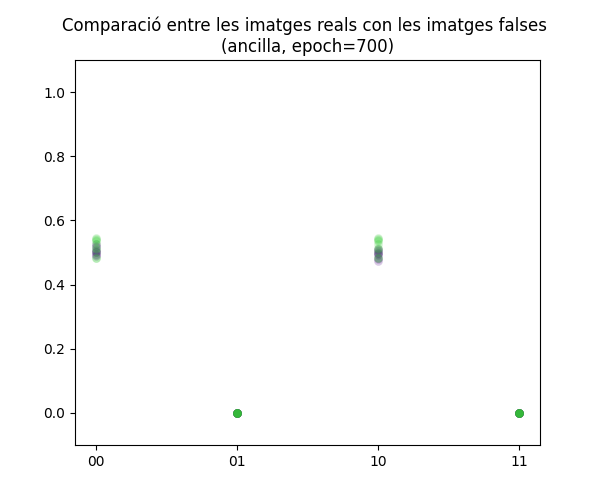
\includegraphics[width=\linewidth]{figures/data/scatter_plot_A4.png}
		\caption{}
	\end{subfigure}
	\begin{subfigure}[b]{.32\linewidth}
		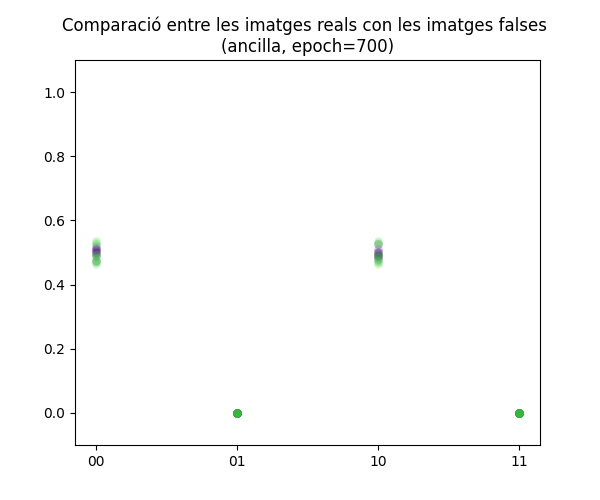
\includegraphics[width=\linewidth]{figures/data/scatter_plot_A5.png}
		\caption{}
	\end{subfigure}
	\begin{subfigure}[b]{.32\linewidth}
		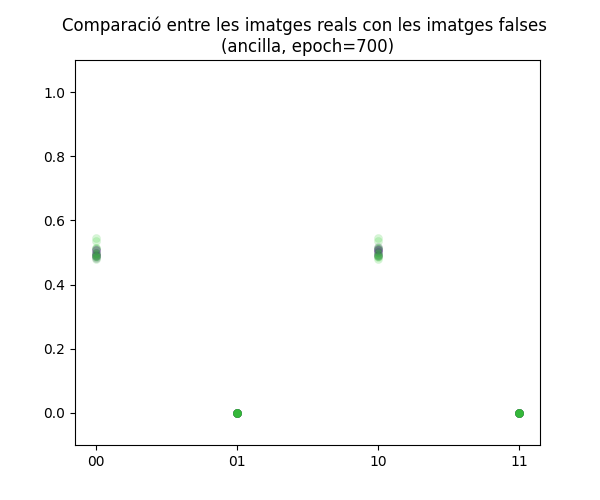
\includegraphics[width=\linewidth]{figures/data/scatter_plot_A6.png}
		\caption{}
	\end{subfigure}
	\label{fig:700_images}
	\caption{Aquestes gràfiques corresponen als mateixos models que els de la figura \ref{fig:700_SD_score}. Les posicions de les gràfiques són les mateixes, per tant, si estan en la mateixa posició que les de l'altra figura, corresponen al mateix model. Les imatges generades pels models sense la funció no-lienal (\textbf{A}, \textbf{C}, \textbf{B}) no s'assemblen a les reals. Es pot veure com els punts de les imatges generades (color violeta) no estan als mateixos valors. Mentre que en les gràfiques \textbf{D}, \textbf{E} i \textbf{F}, sí que ho estan. Els punts violetes sembla que representen la mitjana dels punts verds. També es pot observar que les imatges generades tendeixen a ser més variades que les reals.}
	
\end{figure}



